% 物理学会講演概要集原稿用テンプレート
%		by Hitoshi Nakahara, nakahara@nuqe.nagoya-u.ac.jp
%		Created: 2004/1/7
%		Last Modified: 2004/1/15
%
% ※ 本ファイルの配布、改変等は自由に行っていただいて構いません。
% ※ 作者は本ファイルの動作を保証するものではありません。
% ※ 自らの責任に於いて使用してください。
% ※ 内容に関する質問にはお答えできないことがあります。

\documentclass[12pt, a4paper]{jarticle}
%\usepackage{citesort}
\usepackage{amssymb}
\usepackage[dvipdfmx]{graphicx}		% 図を入れるときに使用
\usepackage{wrapfig}		% 図の周りに本文を流し込みたいときに使用
% 使用例
% \begin{wrapfigure}{r}{8cm}
% \includegraphics[width=8cm]{apparatus.eps}
% \caption{これは図のキャプションです。}
% \end{wrapfigure}
% 流し込みたい段落が続く...

%%%%% 以下のヘッダ項目を変更してください (前後に余分なスペースは入れないでください)
%% 必要に応じて改行 "\\" 等のコマンドを含めて構いません

\newcommand{\講演番号}
{}

\newcommand{\講演題目}
{非調和振動の効果を入れた有限温度自由エネルギー計算}

\newcommand{\英文題目}
{Free energy calculation of finite temperature with anharmonic effects.}

\newcommand{\和文所属}
{関西学院大・理工}

\newcommand{\和文氏名}
{榊原健,西谷滋人}

\newcommand{\英文所属}
{Department of Informatics, Kwansei Gakuin Univ}

\newcommand{\英文氏名}
{K. Sakakibara, S. R. Nishitani}

%% ヘッダ項目、ここまで

%%%%% 新規変数の定義、変更しないでください
\newlength\題目幅
\newlength\ヘッダ項目間隔
\newlength\所属インデント
\newlength\和文氏名インデント
\newlength\英文氏名インデント
\newlength\最小所属氏名間隔
\newlength\ヘッダ行間隔
\newlength\本文行間隔
\newlength\上端余白
\newlength\左端余白
\newlength\idWidth
\newlength\titleNoSpacing
\newlength\autherWidth
\newlength\affilWidthJ
\newlength\affilWidthE
\newcount\crAuthorJ
\newcount\crAuthorE
\newcount\和文氏名を右揃
\newcount\英文氏名を右揃

%%%%% 以下の数値は適宜変更してください
\setlength\題目幅{133mm}				% 題目の幅、125〜130mmが適切です
\setlength\所属インデント{17mm}			% 左端から所属を開始する位置までの長さ、15〜20mmが適切です
\setlength\和文氏名インデント{55mm}		% 和文氏名の開始位置 (所属インデント位置からの長さ)
%\setlength\和文氏名インデント{5mm}		% 和文氏名の開始位置 (所属インデント位置からの長さ)
\setlength\英文氏名インデント{55mm}		% 英文氏名の開始位置 (所属インデント位置からの長さ)
\setlength\最小所属氏名間隔{1ex}			% 氏名と所属の間の最小間隔 (これ以下になると氏名を改行します)
\setlength\ヘッダ行間隔{6mm plus .3mm minus .3mm}		% ヘッダ項目の行間、6〜7mmが適切です
\setlength\ヘッダ項目間隔{1.5mm}						% ヘッダ項目間に追加する間隔、1〜2mmが適切です
\setlength\本文行間隔{7.5mm plus .5mm minus 1mm}		% 本文の行間、7〜8mmが適切です
\setlength\上端余白{15mm}							% 出力機器に依存します
\setlength\左端余白{16.5mm}							% 出力機器に依存します
\和文氏名を右揃 = 1				% 和文氏名を右寄せにするときは1、インデント位置に揃えるときは0
\英文氏名を右揃 = 1					% 英文氏名を右寄せにするときは1、インデント位置に揃えるときは0

%%%%% ここから本文入力位置までは通常は変更の必要はありません

\setlength{\textwidth}{168mm}	% 印刷領域の幅
\setlength{\textheight}{254mm}	% 印刷領域の高さ
\setlength{\topmargin}{-1in}
\setlength{\headheight}{0mm}
\setlength{\textfloatsep}{4mm}	% 図と文章のマージン
\setlength{\idWidth}{30mm}		% 講演番号の幅
\crAuthorJ = 0
\crAuthorE = 0

%%%%% 必要な間隔を計算
\setlength{\headsep}{\上端余白}
\setlength{\oddsidemargin}{-1in}
\addtolength{\oddsidemargin}{\左端余白}
\setlength{\evensidemargin}{\oddsidemargin}
\setlength{\titleNoSpacing}{\textwidth}
\addtolength{\titleNoSpacing}{-1\idWidth}
\addtolength{\titleNoSpacing}{-1\題目幅}
\setlength{\autherWidth}{\textwidth}
\addtolength{\autherWidth}{-1\所属インデント}

% 動的に決まる長さを計算
\setbox0 = \hbox{\和文所属}
\setlength{\affilWidthJ}{\wd0}
\setbox1 = \hbox{\英文所属,}
\setlength{\affilWidthE}{\wd1}
\addtolength{\affilWidthJ}{\最小所属氏名間隔}
\addtolength{\affilWidthE}{\最小所属氏名間隔}
\ifdim\affilWidthJ<\和文氏名インデント
\addtolength{\和文氏名インデント}{-1\wd0}
\else
\crAuthorJ = 1	% 所属が長いときは氏名の前で改行
\fi
\ifdim\affilWidthE<\英文氏名インデント
\addtolength{\英文氏名インデント}{-1\wd1}
\else
\crAuthorE = 1	% 所属が長いときは氏名の前で改行
\fi

%%%%% その他の設定
\renewcommand\refname{\vspace{-15mm}}		% 参考文献のタイトルは表示はしない

% ドキュメント開始、ヘッダ項目の表示
\begin{document}
\thispagestyle{empty}
\pagestyle{empty}


\setlength\parindent{0mm}
\vrule width 0mm height 6mm depth 5mm				% タイトルの高さをキープするためのダミー
\parbox{\idWidth}{\setlength\baselineskip{\ヘッダ行間隔}
{\hfil\small\tt\講演番号\hfil}}\hspace{\titleNoSpacing}%
\parbox{\題目幅}{{\fontsize{16pt}{0pt}\selectfont{\bf\講演題目}}}\par


\vspace{\ヘッダ項目間隔}\hspace*{\所属インデント}%
\parbox{\autherWidth}{\setlength\baselineskip{\ヘッダ行間隔}
{\bf{\fontsize{14pt}{0pt}\selectfont{\和文所属}}}%
\ifnum\crAuthorJ = 0
\ifnum\和文氏名を右揃 = 0
\hspace{\和文氏名インデント}{\bf{\fontsize{14pt}{0pt}\selectfont{\和文氏名}}}%
\else
\hfill{\和文氏名}%
\fi
\else
\ifnum\英文氏名を右揃 = 0
\\\hspace{\和文氏名インデント}{\bf{\fontsize{14pt}{0pt}\selectfont{\和文氏名}}}%
\else
\\\hfill{\bf{\fontsize{14pt}{0pt}\selectfont{\和文氏名}}}%
\fi
\fi
}\par

\vspace{\ヘッダ項目間隔}\hspace*{\所属インデント}%
\parbox{\autherWidth}{\setlength\baselineskip{\ヘッダ行間隔}{\bf{\fontsize{14pt}{0pt}\selectfont{\英文題目}}}}\par

\vspace{\ヘッダ項目間隔}\hspace*{\所属インデント}%
\parbox{\autherWidth}{\setlength\baselineskip{\ヘッダ行間隔}
{\it{\fontsize{14pt}{0pt}\selectfont{\英文所属}}},%
\ifnum\crAuthorE = 0
\ifnum\英文氏名を右揃 = 0
\hspace{\英文氏名インデント}{\bf{\fontsize{14pt}{0pt}\selectfont{\英文氏名}}}%
\else
\hfill{\bf{\fontsize{14pt}{0pt}\selectfont{\英文氏名}}}%
\fi
\else
\ifnum\英文氏名を右揃 = 0
\\\hspace{\英文氏名インデント}{\bf{\fontsize{14pt}{0pt}\selectfont{\英文氏名}}}%
\else
%\\\hfill
\\{\bf{\fontsize{14pt}{0pt}\selectfont{\英文氏名}}}%なぜかここ動いてる
\fi
\fi
}\par



\setlength\parindent{1zw}\setlength\baselineskip{\本文行間隔}
\vspace*{\本文行間隔}


%%%%% 以下の部分に本文を入力してください %%%%%

\paragraph{}
材料設計において系の有限温度における自由エネルギーの変化は重要である.
第一原理計算ソフトVASP(Vienna ab initio simulation package)では,擬調和振動子近似に基づいたphonon計算パッケージが開発されており,自由エネルギーを見積もることができる\cite{phonon}.
しかし,Ti結晶での相変態温度近傍での振る舞いにおいて理想の結果が得られず,これは非調和の項の影響が大きいからだと思われる.
\paragraph{}
神藤のMoment法では,有限温度における自由エネルギー,熱膨張などを見積もることができる\cite{jindo}.図1,2はfcc構造の金属であるCu, Ag, Auのシミュレーション結果であり,自由エネルギー,最近接原子間距離が温度に上手く依存していることが確認できる.しかし,ポテンシャルの2次,4次微分を利用するこの計算手法の正当性はわかっておらず検証を行う必要がある.
また,単純なペアポテンシャルを利用しているがVASPでの計算結果の組み込みが可能か検証を行う.



%\begin{wrapfigure}{r}{8.8cm}
\begin{center}
\begin{figure}[h]
\begin{minipage}{0.5\hsize}
\begin{center}
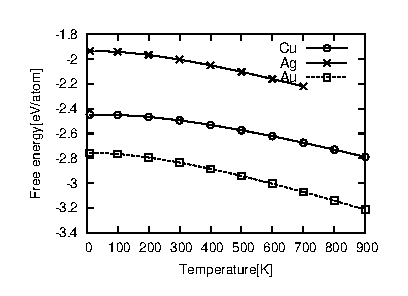
\includegraphics[width=8.8cm]{./energy.eps}
\caption{\small{Cu, Ag, Auにおける自由エネルギーの温度依存性.}}
\end{center}
\end{minipage}
\hspace{5mm}
\begin{minipage}{0.5\hsize}
\begin{center}
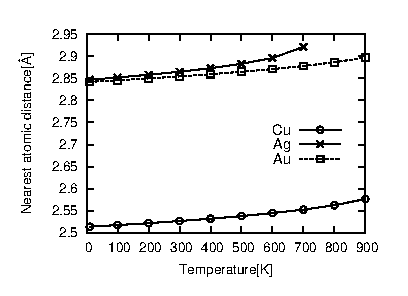
\includegraphics[width=8.8cm]{./distance.eps}
\caption{\small{Cu, Ag, Auにおける最近接原子間距離の温度依存性.}}
\end{center}
\end{minipage}
\end{figure}
\end{center}
%\end{wrapfigure}

\smallskip
{\small\setlength\baselineskip{10pt}	% 参考文献は小さめの文字で行間を詰めてある
\begin{thebibliography}{9}
\bibitem{phonon}K. Parlinski, Z. Q. Li and Y. Kawazoe, Phys. Rev. Let., 78, 4063-4066 (1997).
\bibitem{jindo}Vu Van Hung, \& K. Masuda-Jindo, J. Phys. Soc. Jpn. 69 (2000), 2067.
\end{thebibliography}
}

\end{document}
